\documentclass[11pt, twoside]{report}

\usepackage{fontspec}
\usepackage[utf8]{inputenc}
\usepackage[bitstream-charter]{mathdesign}
\usepackage{bbding}
\usepackage{ragged2e}
\usepackage{parskip}
\usepackage{enumitem}
\usepackage{titlesec}
\usepackage{paracol}
\usepackage{mdframed}
\usepackage[margin=1in]{geometry}

\usepackage[autocompile]{gregoriotex}

\titleformat{\chapter}[block]{\huge\scshape\filcenter}{}{1em}{}
\titleformat{\section}[block]{\Large\bfseries\filcenter}{}{1em}{}

\mdfsetup{skipabove=\topskip, skipbelow=\topskip}

\newcommand{\rubric}[1]{
	\switchcolumn[0] {
		\itshape
		#1
	}
}

\newcommand{\latinenglish}[2]{
	\switchcolumn[0]* {
		#1
	}
	\switchcolumn[1] {
		\itshape\small
		#2
	}
}

\newcommand{\latinenglishequal}[2]{
	\switchcolumn[0]* {
		#1
	}
	\switchcolumn[1] {
		\itshape
		#2
	}
}

\newenvironment{latinenglishsection}
	{\columnratio{.7, .3} \begin{paracol}{2}}
	{\end{paracol}}

\newenvironment{latinenglishequalsection}
	{\columnratio{.5, .5}\begin{paracol}{2}}
	{\end{paracol}}

\setlength{\columnseprule}{0.4pt}

\newcommand{\heading}[1]{
	\begin{leftcolumn}
		#1
	\end{leftcolumn}
}

\newcommand{\spanning}[1]{
	\switchcolumn*[#1]
}

\newenvironment{verses}[1]
	{\begin{flushleft} \begin{enumerate}[leftmargin=*] \setcounter{enumi}{#1}}
	{\end{enumerate} \end{flushleft}}

\newenvironment{versicles}{\par\leavevmode\parskip=0pt}{}

\newenvironment{collect}
{
	\leavevmode
	\parindent=1em
	\parskip=0pt
	\noindent Orémus.\par
}{}

\newenvironment{optionbox}
{
	\switchcolumn[0]
	\begin{mdframed}
%	\begin{minipage}{0.8\linewidth}
}{
%	\end{minipage}
	\end{mdframed}
}

\newcommand{\optionrule}{
	\begin{center}
	\rule{0.5\linewidth}{0.6pt}
	\end{center}
}

\newenvironment{optionruled}
{
	\optionrule
}
{
	\optionrule
}

% for use inside the collect environment
\newcommand{\Amen}{\par\noindent \Rbar. Amen.}

\begin{document}

\vspace*{2cm}

\begin{center}
	\textbf{\Huge Vespers of the Blessed Virgin Mary}\\
	{\LARGE According to the Washtenaw Use}
\end{center}

\vspace*{1cm}
%\maketitle

\begin{center}
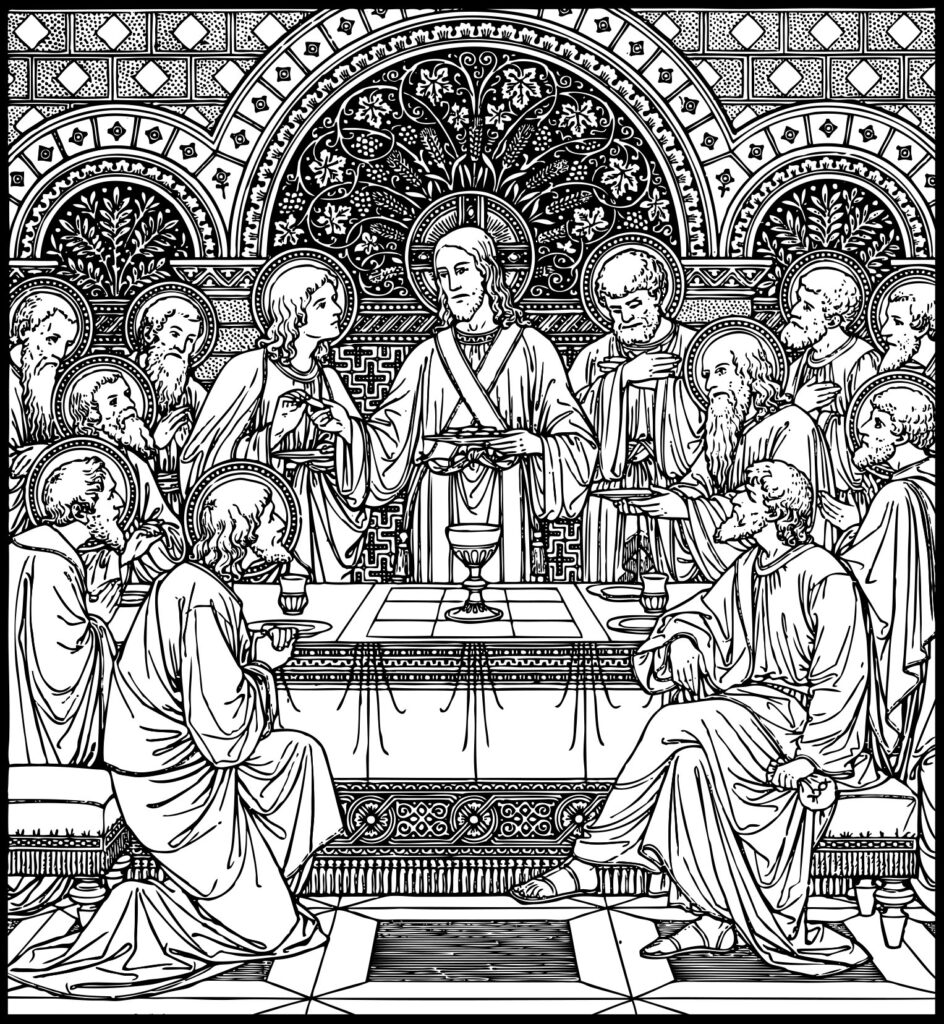
\includegraphics[width=0.75\textwidth]{ChristLastSupper}
\end{center}

\hspace{0pt}
\vfill

\pagebreak

\vspace*{7.5cm}
``At \textit{Evensong} time, Our Lord Jesus Christ on Maundy Thursday supped with His Apostles, and ordained the Holy Sacrament of His Body and Blood. The same hour on Good Friday, He was taken down from The Cross. And on Easter Day, the same hour, He met with two of His disciples going towards Emmaus, and made Himself known to them in the breaking of bread.'' (Paraphrased from the \textit{Mirror of Our Lady}.) O most blessed Virgin, you grieved bitterly as your divine son's body was lowered from The Cross, having wrought fo us our redemption; pray that we may ever be mindful that the same glorious body is given to us in the Holy Eucharist and always treat this Sacrament with due reverence. Amen.
\vfill

\pagebreak

\chapter*{Before Vespers}

\section*{Preparatory Prayers}

\textit{ All kneel and pray silently. As you say the prayer \textnormal{Aperi, Domine}, make the sign of the cross with your thumb first over your lips, and then over your heart.}

\begin{latinenglishequalsection}

\latinenglishequal{
	Áperi, {\color{red}\maltese}\ Dómine, os meum ad benedicéndum\linebreak nomen sanctum tuum:
	{\color{red}\maltese}\ munda quoque cor meum ab ómnibus vanis, pervérsis et aliénis cogitatiónibus;
	intelléctum illúmina, afféctum inflámma, ut digne, atténte ac devóte hoc Offícium beátæ Vírginis Maríæ recitáre váleam,
	et exaudíri mérear ante conspéctum divínæ Majestátis tuæ.
	Per Christum Dóminum nostrum. 
	Amen.
}{
	Open, {\color{red}\maltese}\ O Lord, my mouth to bless Thy holy Name; {\color{red}\maltese}\ cleanse also my heart from all vain, evil, and wandering thoughts; enlighten my understanding and kindle my affections; that I may worthily, attentively, and devoutly say this Office of the Blessed Virgin Mary, and so merit to be heard before the presence of Thy divine Majesty.  Through Christ our Lord.  Amen.
}

\latinenglishequal{
	Domine, in unióne illíus divínæ intentiónis, qua ipse in terris laudes Deo persolvísti, has tibi Horas persólvo.
}{
	O Lord, in union with that divine intention wherewith thou, whilst here on earth, didst render praises unto God, I desire to offer this my Office of prayer unto thee.
}

\latinenglishequal{
	Pater Noster, qui es in cælis, sanctificétur nomen tuum.
	Advéniat regnum tuum.
	Fiat volúntas tua, sicut in cælo et in terra.
	Panem nostrum quoti\-diánum da nobis hódie,
	et dimítte nobis débita nostra, sicut et nos dimíttimus debitóribus nostris.
	Et ne nos indúcas in tentatiónem: sed líbera nos a malo.
	Amen.
}{
	Our Father, who art in heaven, hallowed be thy name.
	Thy kingdom come.
	Thy will be done, on earth as it is in heaven.
	Give us this day our daily bread, and forgive us our trespasses, as we forgive those who trespass against us.
	And lead us not into temptation: but deliver us from evil.
	Amen.
}

\latinenglishequal{
	Ave María, grátia plena, Dóminus tecum. Benedíc\-ta tu in muliéribus, et benedíctus fructus ventris tui, Jesus.
 Sancta María, Mater Dei, ora pro nobis peccatóribus, nunc et in hora mortis nostræ. Amen.
 }{
 	Hail Mary, full of grace, the Lord is with thee. Blessed art thou among women, and blessed is the fruit of thy womb, Jesus.
 Holy Mary, Mother of God, pray for us sinners, now and at the hour of our death. Amen.
 }
 
 \end{latinenglishequalsection}

\chapter*{Vespers}

\begin{latinenglishsection}

\rubric{\color{red}All make the Sign of the Cross as the Officiant says (All continue together with the entire ``Gloria Patri'' after the response): }

\latinenglish{
	\gresetinitiallines{1}
	\gregorioscore{deus_in_adjutorium}
}{
	O God, come to my assistance.
		
	O Lord, make haste to help me.
	
	Glory be to the Father, and to the Son, and to the Holy Spirit,
	as it was in the beginning, is now, and ever shall be, world without end. Amen.
	
	Alleluia.
}

\rubric{\color{red}From Septuagesima until Easter, \textnormal{Alleluia} is replaced with:}

\latinenglish{
	\gresetinitiallines{0}
	\gabcsnippet{
	(c3)Lau(h)s ti(h)bi(h) Dó(h)mi(h)ne(h), Re(h)x æ(h)té(h)rné(i) gló(h)ri(h)æ(g). (::)
	}
}{
	Praise to thee, O Lord, King of everlasting glory.
}

\rubric{\color{red} For `Throughout the Year', \underline{see page 5}.}
\rubric{\color{red} For `Advent', \underline{see page 14}.}
\rubric{\color{red} For `Christmastide', \underline{see page 22}.}

\end{latinenglishsection}

\pagebreak

\section*{THROUGHOUT THE YEAR}
\noindent\textit{\color{red}Note that in Paschal Time, the Alleluia is chanted after the antiphon following each Psalm, and the Magnificat antiphon changes to Regina Caeli.}

\begin{latinenglishsection}

% Psalm cix: Dixit Dominus (with antiphon)

\heading{\section*{Psalm 109}}

\rubric{\color{red}The Cantor intones the antiphon and leads the first Psalm verse to the star (*). All sit, while the Cantor's side finishes the first verse together. The Officiants side then says the second Psalm verse, with each side alternating thereafter. All say the antiphon together at the end.}


\latinenglish{
	\gresetinitiallines{1}
	\gregorioscore{dum_esset_intonation}
}{
	While the king...
}

\latinenglish{
	\gresetinitiallines{0}
	\gregorioscore{psalm_109_1_3a}
	
	\begin{verses}{1}
	
	\item Donec ponam ini\textbf{mí}cos \textbf{tu}os, *\\
	scabéllum pedum \textit{tu}\textbf{ó}rum.
	
	\item Virgam virtútis tuæ emíttet Dómi\textbf{nus} ex \textbf{Si}on: *\\
	domináre in médio inimicórum \textit{tu}\textbf{ó}rum.
	
	\item Tecum princípium in die virtútis tuæ in splendóri\textbf{bus} sanc\textbf{tó}rum: *\\
	ex útero ante lucíferum gé\textit{nu}\textbf{i} te.
	
	\item Jurávit Dóminus, et non pœni\textbf{té}bit \textbf{e}um: *\\
	Tu es sacérdos in ætérnum secúndum órdinem \textit{Mel}\textbf{chí}sedech.
	
	\item Dóminus a \textbf{dex}tris \textbf{tu}is, *\\
	confrégit in die iræ su\textit{æ} \textbf{re}ges.
	
	\item Judicábit in natiónibus, im\textbf{plé}bit ru\textbf{í}nas: *\\
	conquassábit cápita in terra \textit{mul}\textbf{tó}rum.
	
	\item De torrénte in \textbf{vi}a \textbf{bi}bet: *\\
	 {\color{red}\textit{(stand)}} proptérea exaltá\textit{bit} \textbf{ca}put.
	
	\item  {\color{red}\textit{(bow)}} Glória \textbf{Pa}tri, et \textbf{Fíli}o, *\\
	et Spirítu\textit{i} \textbf{Sanc}to.
	
	\item  {\color{red}\textit{(rise)}} Sicut erat in princípio, et \textbf{nunc}, et \textbf{sem}per, *\\
	et in s\'{\ae}cula sæculó\textit{rum}. \textbf{A}men.
	
	\end{verses}
	\pagebreak
	
	\gresetinitiallines{1}
	\gregorioscore{dum_esset}
}{
	1. The Lord said to my Lord: Sit thou at my right hand:
	
	2. Until I make thine enemies: thy footstool.
	
	3. The Lord shall send forth the rod of thy power from out of Sion: rule thou in the midst of thine enemies.
	
	4. Thine shall be the dominion in the day of thy power, amid the brightness of the saints: from the womb, before the day-star, have I begotten thee.
	
	5. The Lord hath sworn, and will not repent: Thou art a priest for ever according to the order of Melchisedech.
	
	6. The Lord upon thy right hand: hath overthrown kings in the day of his wrath.
	
	7. He shall judge among the nations, he shall fulfill destructions: he shall smit in sunder the heads in the land of many.
	
	8. He shall drink of the brook in the way: therefore shall he lift of up his head.
	
	9. Glory be to the Father, and to the Son, and to the Holy Spirit.
	
	10. As it was in the beginning, is now, and shall be forever. Amen.
	
	While the King was reposing, my spikenard yielded the odour of sweetness.
}

\rubric{\color{red}The remaining antiphons and psalms are sung in the same manner as the first.}

% Psalm cxii: Laudate, pueri (with antiphon)

\heading{\section*{Psalm 112}}

\latinenglish{
	\gresetinitiallines{1}
	\gregorioscore{læva_ejus_intonation}
}{
	His left hand...
}

\latinenglish{
	\gresetinitiallines{0}
	\gregorioscore{psalm_112_1_4A_STAR}
	
	\begin{verses}{1}
	
	\item Sit nomen Dómini \textit{bene}\textbf{díc}tum, *\\
	ex hoc nunc, et \textit{usque} \textit{in} \textit{sæ}cu\textbf{lum}.
	
	\item A solis ortu usque \textit{ad} \textit{oc}\textbf{cá}sum, *\\
	laudábi\textit{le} \textit{nomen} \textbf{Dó}mini.
	
	\item Excélsus super omnes \textit{gentes} \textbf{Dó}minus, *\\
	et super cælos \textit{glória} \textbf{e}jus.
	
	\item Quis sicut Dóminus, Deus noster, qui in \textit{altis} \textbf{há}bitat, *\\
	et humília réspicit in cæ\textit{lo} \textit{et} \textit{in} \textbf{ter}ra?
	
	\item Súscitans a \textit{terra} \textbf{ín}opem, *\\
	et de stércore \textit{érigens} \textbf{páu}perem:
	
	\item Ut cóllocet eum \textit{cum} \textit{prin}\textbf{cí}pibus, *\\
	cum princípibus \textit{pópuli} \textbf{su}i.
	
	\item Qui habitáre facit stéri\textit{lem} \textit{in} \textbf{do}mo, *\\
	 {\color{red}\textit{(stand)}} matrem fili\textit{órum} \textit{læ}\textbf{tán}tem.
	
	\item  {\color{red}\textit{(bow)}} Glória Pa\textit{tri}, \textit{et} \textbf{Fí}lio, *\\
	et Spi\textit{rítui} \textbf{Sanc}to.
	
	\item  {\color{red}\textit{(rise)}} Sicut erat in princípio, et \textit{nunc}, \textit{et} \textbf{sem}per, *\\
	et in s\'{\ae}cula sæ\textit{culórum}. \textbf{A}men.
	
	\end{verses}
	
	\pagebreak
	
	\gresetinitiallines{1}
	\gregorioscore{læva_ejus}
}{
	1. Praise the Lord, ye children: praise ye the name of the Lord:
	
	2. Blessed be the name of the Lord: from this time forth, forevermore.
	
	3. From the rising up of the sun unto the going down of the sameL the name of the Lord is worthy to be praised.
	
	4. The Lord is high above all nations: and his glory above the heavens.
	
	5. Who is like unto the Lord our God, who dwelleth on high: and regardeth the things that are lowly in heaven and on earth?
	
	6. Who raiseth up the needy from the earth: and lifteth the poor from off the dunghill.
	
	7. That he may set him with the princes: even with the princes of his people.
	
	8. Who maketh the barren woman to dwell in her houseL the joyful mother of children.
	
	9. Glory be to the Father, and to the Son, and to the Holy Spirit.
	
	10. As it was in the beginning, is now, and shall be forever. Amen.
	
	His left hand under my head, and his right hand shall embrace me.
}

\end{latinenglishsection}

\begin{latinenglishsection}

% Psalm cxxi: Lætatus sum in his (with antiphon)

\heading{\section*{Psalm 121}}

\latinenglish{
	\gresetinitiallines{1}
	\gregorioscore{nigra_sum_intonation}
}{
	I am black but beautiful...
}

\latinenglish{
	\gresetinitiallines{0}
	\gregorioscore{psalm_121_1_3b}
	
	\begin{verses}{1}
	
	\item Stantes erant \textbf{pe}des \textbf{no}stri, *\\
	in átriis tuis, \textit{Je}\textbf{rú}salem.
	
	\item Jerúsalem, quæ ædifi\textbf{cá}tur ut \textbf{cívi}tas: *\\
	cujus participátio ejus in \textit{id}\textbf{íp}sum.
	
	\item Illuc enim ascendérunt \textbf{tri}bus, tribus \textbf{Dómi}ni: *\\
	testimónium Israël ad confiténdum nómi\textit{ni} \textbf{Dó}mini.
	
	\item Quia illic sedérunt sedes \textbf{in} ju\textbf{díci}o, *\\
	sedes super do\textit{mum} \textbf{Da}vid.
	
	\item Rogáte quæ ad pacem \textbf{sunt} Je\textbf{rúsa}lem: *\\
	et abundántia diligén\textit{ti}\textbf{bus} te:
	
	\item Fiat pax in vir\textbf{tú}te \textbf{tu}a: *\\
	et abundántia in túrri\textit{bus} \textbf{tu}is.
	
	\item Propter fratres meos, et \textbf{pró}ximos \textbf{me}os, *\\
	loquébar pa\textit{cem} \textbf{de} te:
	
	\item Propter domum Dómini, \textbf{De}i \textbf{nos}tri, *\\
	{\color{red}\textit{(stand)}} quæsívi bo\textit{na} \textbf{ti}bi.
	
	\item {\color{red}\textit{(bow)}} Glória \textbf{Pa}tri, et \textbf{Fíli}o, * \\
	et Spirítu\textit{i} \textbf{Sanc}to.
	
	\item {\color{red}\textit{(rise)}} Sicut erat in princípio, et \textbf{nunc}, et \textbf{sem}per, *\\
	et in s\'{\ae}cula sæculó\textit{rum}. \textbf{A}men.
	
	\end{verses}
	
	\pagebreak
	
	\gresetinitiallines{1}
	\gregorioscore{nigra_sum}
}{
	1. I was glad at the things that were said unto me : We will go into the house of the Lord.
	
	2. Our feet were wont to stand: in thy courts, O Jerusalem.
	
	3. Jerusalem, which is built as a city: that is at unity with itself.
	
	4. For thither did the tribes go up, the tribes of the Lord: the testimony of Israel, to praise the name of the Lord.
	
	5. For there are set the seats of judgement: the seats over the house of David.
	
	6. Pray ye for the things that are for the peace of Jerusaelm: and plenteousness be to them that love thee.
	
	7. Let peace be in thy strength: and plenteousness in thy towers.
	
	8. For my brethren and companions' sake: I spake peace concerning thee.
	
	9. Because of the house of the Lord our God: I have sought good things for thee.
	
	10. Glory be to the Father, and to the Son, and to the Holy Spirit.
	
	11. As it was in the beginning, is now, and shall be forever. Amen.
	
	I am black, but beautiful, O daughters of Jerusalem: therefore hath the king loved me, and brought me into his chamber.
}

\end{latinenglishsection}

\begin{latinenglishsection}

% Psalm cxxvi: Nisi Dominus (with antiphon)

\heading{\section*{Psalm 126}}

\latinenglish{
	\gresetinitiallines{1}
	\gregorioscore{jam_hiems_intonation}
}{
	Now is the winter past...
}

\latinenglish{
	\gresetinitiallines{0}
	\gregorioscore{psalm_126_1_8G}
	
	\begin{verses}{1}
	
	\item Nisi Dóminus custodíerit civi\textbf{tá}tem, *\\
	frustra vígilat qui cus\textit{tódit} \textbf{e}am.
	
	\item Vanum est vobis ante lucem \textbf{súr}gere: *\\
	súrgite postquam sedéritis, qui manducátis pa\textit{nem} \textit{do}\textbf{ló}ris.
	
	\item Cum déderit diléctis suis \textbf{som}num: *\\
	ecce heréditas Dómini fílii : merces, \textit{fructus} \textbf{ven}tris.
	
	\item Sicut sagíttæ in manu pot\textbf{én}tis: *\\
	ita fílii \textit{excus}\textbf{só}rum.
	
	\item Beátus vir qui implévit desidérium suum ex \textbf{ip}sis: *\\
	{\color{red}\textit{(stand)}} non confundétur cum loquétur inimícis su\textit{is} \textit{in} \textbf{po}rta.
	
	\item {\color{red}\textit{(bow)}} Glória Patri, et \textbf{Fí}lio, * \\
	et Spirí\textit{tui} \textbf{Sanc}to.
	
	\item {\color{red}\textit{(rise)}} Sicut erat in princípio, et nunc, et \textbf{sem}per, *\\
	et in s\'{\ae}cula sæcu\textit{lórum}. \textbf{A}men.
	
	\end{verses}
	
	\pagebreak
	
	\gresetinitiallines{1}
	\gregorioscore{jam_hiems}
}{
	1. Unless the Lord build the house: they labour in vain that build it.
	
	2. Unless the Lord keep the city: he watcheth in vain that keepeth it.
	
	3. In vain ye rise before the light: rise not till ye have rested, O ye that eat the bread of sorrow.
	
	4. When he hath given sleep to his beloved: lo, children are a heritage from the Lord, and the fruit of the womb a reward.
	
	5. Like as arrows in the hand of the mighty one: so are the children of those who have been cast out.
	
	6. Blessed is the man whose desire is satisfied with the: he shall not be confounded, when he speaketh with his enemies in the gate.
	
	7. Glory be to the Father, and to the Son, and to the Holy Spirit.
	
	8. As it was in the beginning, is now, and shall be forever. Amen.
	
	Now is the winter past, the rain is over and gone: arise, my beloved, and come.
}

\end{latinenglishsection}

\begin{latinenglishsection}

% Psalm cxlvii: Lauda Jerusalem (with antiphon)

\heading{\section*{Psalm 147}}

\latinenglish{
	\gresetinitiallines{1}
	\gregorioscore{speciosa_facta_intonation}
}{
	Thou art become beautiful...
}

\latinenglish{
	\gresetinitiallines{0}
	\gregorioscore{psalm_147_1_4A_STAR}
	
	\begin{verses}{1}
	
	\item Quóniam confortávit seras portá\textit{rum tu}\textbf{á}rum: * \\
	benedíxit fíli\textit{is tuis} \textbf{in} te.
	
	\item Qui pósuit fines \textit{tuos} \textbf{pa}cem: * \\
	et ádipe frumén\textit{ti sáti}\textbf{at} te.

	\item Qui emíttit elóquium \textit{suum} \textbf{ter}ræ : * \\
	velóciter cur\textit{rit sermo} \textbf{e}jus.
	
	\item Qui dat nivem \textit{sicut} \textbf{la}nam: * \\
	nébulam sicut \textit{cínerem} \textbf{spar}git.
	
	\item Mittit crystállum suam sic\textit{ut buc}\textbf{cél}las: * \\
	ante fáciem frígoris ejus \textit{quis susti}\textbf{né}bit?
	
	\item Emíttet verbum suum, et liquefá\textit{ciet} \textbf{e}a: * \\
	flabit spíritus ejus, \textit{et fluent} \textbf{a}quæ.
	
	\item Qui annúntiat verbum \textit{suum} \textbf{Ja}cob: * \\
	justítias, et judíci\textit{a sua} \textbf{Is}raël.
	
	\item Non fecit táliter omni \textit{nati}\textbf{ó}ni: * \\
	{\color{red}\textit{(stand)}} et judícia sua non mani\textit{festávit} \textbf{e}is.
	
	\item {\color{red}\textit{(bow)}} Glória Pa\textit{tri, et} \textbf{Fí}lio, * \\
	et Spi\textit{rítui} \textbf{Sanc}to.
	
	\item {\color{red}\textit{(rise)}} Sicut erat in princípio, et \textit{nunc, et} \textbf{sem}per, * \\
	et in s\'{\ae}cula sæ\textit{culórum}. \textbf{A}men.
	
	\end{verses}
	
	\pagebreak
	
	\gresetinitiallines{1}
	\gregorioscore{speciosa_facta}
}{
	1. Praise the Lord, O Jerusalem: praise thy God, O Sion.
	
	2. For he hath strenghtened the bars of thy gates: he hath blessed hty children within thee.
	
	3. He hath made peace within thy borders: and filleth thee with the fatness of corn.
	
	4. He sendeth forth his commandment on the earth: his word runneth very swiftly.
	
	5. He giveth snow like wool: he scattereth the hoar-frost like ashes.
	
	6. He sendeth his ice like morsels: who is able to abide his frost?
	
	7. He shall send fort his word, and melt them: he shall blow with his wind, and the waters shall flow.
	
	8. He maketh known his word unto Jacob: his statues and ordinances unto Israel.
	
	9. He hath not dealt so with any nation: neither hath he shewed them his judgements.
	
	10. Glory be to the Father and to the Son, and to the Holy Spirit.
	
	11. As it was in the beginning, is now, and shall be forever. Amen.
	
	Thou art become beautiful and sweet in thy delights, O holy Mother of God.
}

\end{latinenglishsection}

\begin{latinenglishsection}

\section*{The Little Chapter: Sirach 24:14}

\rubric{\color{red}The Officiant leads the Little Chapter:}

\latinenglish{
	Ab initio et ante creata sum, {\color{red}\GreDagger}\ et usque ad futurum \textit{non de}\textbf{si}nam, et in habitatione sancta coram ipso ministravi.
	
	{\color{red}\Rbar.} Deo gratias.
}{
	From the beginning, and before the world, was I created, and unto the world to come I shall not cease to be, and in the holy dwelling-place, I have ministered before him.
	
	{\color{red}\Rbar.} Thanks be to God.
}

\end{latinenglishsection}

\begin{latinenglishsection}

\section*{Marian Hymn}

\latinenglish{
	\gresetinitiallines{1}
	\gregorioscore{ave_maris_stella_solemnes}
}{
	1. Gentle Star of the ocean,
	Portal of the sky,
	Ever Virgin Mother,
	Of the Lord Most High.
	
	2. Oh! by Gabriel's Ave,
	Utter'd long ago,
	Eva's name reversing,
	Stablish peace below.
	
	3. Break the captive's fetters,
	Light on blindness pour,
	All our ills expelling,
	Every bliss implore.
	
	4. Shew thyself a Mother,
	Offer him our sigs,
	Who for us Incarnate
	Did not thee despise.
	
	5. Virgin of all virgins,
	To thy shelter take us.
	Gentlest of the gentle,
	Chaste and gentle make us.
	
	6. Still, as on we journey,
	Help our weak endeavour,
	Till with thee and Jesus,
	We rejoice forever.
	
	7. Through the highest heaven,
	To the Almighty Three,
	Father, Son, and Spirit,
	One same Glory be. Amen.
}
\end{latinenglishsection}

\begin{latinenglishsection}

\section*{Oration}

\rubric{\color{red}The Officiant leads the following prayer:}

\latinenglish{
	\gresetinitiallines{0}
	\gabcsnippet{(c3)<c><sp>V/</sp>.</c> Dif(h)fu(h)sa(h) est(h) gra(h)ti(h)a(h) in(h) la(h)bi(h)is(h) tu(h.)is.(f.) (::)}
}{
	{\color{red}\Vbar.} Grace was poured forth on thy lips.
}
\latinenglish{
	\gresetinitiallines{0}
	\gabcsnippet{(c3)<c><sp>R/</sp>.</c> Prop(h)te(h)re(h)a(h) be(h)ne(h)di(h)xit(h) te(h) De(h)us(h) in(h) æ(h)ter(h.)num.(f.) (::)}
}{
	{\color{red}\Rbar.} Therefore hath the Lord blessed thee forever.
}

\end{latinenglishsection}

\vfill\pagebreak

\begin{latinenglishsection}

\section*{The Magnificat}

\rubric{\color{red}All remain standing. The Cantor intones the antiphon. up to the asterisk (*) and then leads the Magnificat. The Magnificat antiphon is that of the Regina cæli during Paschal time. All cross themselves as the Magnificat is started.}

\latinenglish{
	\gresetinitiallines{1}
	\gregorioscore{beata_mater_intonation}
}{
	Blessed Mother...
}
\latinenglish{
	\gresetinitiallines{1}
	\gregorioscore{Magnificat-2}
	
	\begin{verses}{2}
	
	\item \textit{Quia} respéxit humilitátem ancíllæ \textbf{su}æ:~* ecce enim ex hoc beátam me dicent omnes genera\textit{ti}\textbf{ó}nes.

	\item \textit{Quia} fecit mihi magna qui \textbf{pot}ens est:~* et sanctum no\textit{men} \textbf{e}jus.
	
	\item \textit{Et mi}sericórdia ejus a progénie in pro\textbf{gé}nies~* timénti\textit{bus} \textbf{e}um.
	
	\item \textit{Fecit} poténtiam in bráchio \textbf{su}o:~* dispérsit supérbos mente cor\textit{dis} \textbf{su}i.
	
	\item \textit{Depó}suit poténtes de \textbf{se}de,~* et exaltá\textit{vit} \textbf{hú}miles.
	
	\item \textit{Esu}riéntes implévit \textbf{bo}nis:~* et dívites dimísit \textit{in}\textbf{á}nes.
	
	\item \textit{Suscé}pit Israël púerum \textbf{su}um,~* recordátus misericórdi\textit{æ} \textbf{su}æ.
	
	\item \textit{Sicut} locútus est ad patres \textbf{nos}tros,~* Abraham et sémini ejus \textit{in} \textbf{s\'{\ae}}cula.
	
	\item {\color{red}(bow)} \textit{Glóri}a Patri, et \textbf{Fí}lio,~* et Spirítu\textit{i} \textbf{Sanc}to.
	
	\item {\color{red}(rise)} \textit{Sicut} erat in princípio, et nunc, et \textbf{sem}per,~* et in s\'{\ae}cula sæculó\textit{rum}. \textbf{A}men.
	
	\end{verses}
	
	\gresetinitiallines{0}
	\gregorioscore{beata_mater}
}{
	My soul doth magnify:
	{\color{red}\maltese}\ the Lord.
	
	And my spirit hat rejoiced: 
	in God my Saviour.
	
	For he hath regarded the lowliness of his handmaid:
	for behold from henceforth all generations shall call me blessed.
	
	For he that is mighty hath done great things unto me:
	and holy is His name.
	
	And His mercy is from generation to generation: 
	unto the that fear Him.
	
	He hath shewed strength with His arm:
	he hath scattered the proud in the imagination of their heart.
	
	He hath put down the mighty from their seat:
	and hath exalted the humble.
	
	He hath filled the hungry with good things:
	and the rich he hath sent away empty.
	
	He hath holpen his servant Israel:
	being mindful of His mercy.
	
	As he spake unto our fathers: 
	to Abraham and his seed forever.
	
	Glory be to the Father, and to the Son
	and to the Holy Spirit,
	
	As it was in the beginning, is now,
	and every shall be, world without end, Amen.
	
	Blessed Mother and inviolate Virgin, glorious Queen of the world, intercede or us with the Lord.
}

\end{latinenglishsection}

\vfill\pagebreak

\begin{latinenglishsection}

\rubric{\color{red}In Paschal time, the following is sung:}

\latinenglish{
	\gresetinitiallines{1}
	\gregorioscore{regina_caeli_intonation}
	
	\gresetinitiallines{1}
	\gregorioscore{Magnificat-6}
	
	\begin{verses}{2}
	
	\item \textit{Quia} respéxit humilitátem an\textbf{cíl}læ \textbf{su}æ:~* ecce enim ex hoc beátam me dicent omnes gene\textit{ra}\textit{ti}\textbf{ó}nes.

	\item \textit{Quia} fecit mihi \textbf{ma}gna qui \textbf{pot}ens est:~* et sanctum \textit{no}\textit{men} \textbf{e}jus.
	
	\item \textit{Et mi}sericórdia ejus a progénie \textbf{in} pro\textbf{gé}nies~* timén\textit{ti}\textit{bus} \textbf{e}um.
	
	\item \textit{Fecit} poténtiam in \textbf{brá}chio \textbf{su}o:~* dispérsit supérbos mente \textit{cor}\textit{dis} \textbf{su}i.
	
	\item \textit{Depó}suit pot\textbf{én}tes de \textbf{se}de,~* et exal\textit{tá}\textit{vit} \textbf{hú}miles.
	
	\item \textit{Esu}riéntes im\textbf{plé}vit \textbf{bo}nis:~* et dívites dimí\textit{sit} \textit{in}\textbf{á}nes.
	
	\item \textit{Suscé}pit Israël \textbf{pú}erum \textbf{su}um,~* recordátus misericór\textit{di}\textit{æ} \textbf{su}æ.
	
	\item \textit{Sicut} locútus est ad \textbf{pa}tres \textbf{nos}tros,~* Abraham et sémini e\textit{jus} \textit{in} \textbf{s\'{\ae}}cula.
	
	\item {\color{red}(bow)} \textit{Glóri}a \textbf{Pa}tri, et \textbf{Fí}lio,~* et Spirí\textit{tu}\textit{i} \textbf{Sanc}to.
	
	\item {\color{red}(rise)} \textit{Sicut} erat in princípio, et \textbf{nunc}, et \textbf{sem}per,~* et in s\'{\ae}cula sæcu\textit{ló}\textit{rum}. \textbf{A}men.
	
	\end{verses}
	
	\gresetinitiallines{0}
	\gregorioscore{regina_caeli}
}{
	Queen of heaven...
	
	My soul doth magnify:
	{\color{red}\maltese}\ the Lord.
	
	And my spirit hath rejoiced: 
	in God my Saviour.
	
	For he hath regarded the lowliness of his handmaid:
	for behold from henceforth all generations shall call me blessed.
	
	For he that is mighty hath done great things unto me:
	and holy is His name.
	
	And His mercy is from generation to generation: 
	unto the that fear Him.
	
	He hath shewed strength with His arm:
	he hath scattered the proud in the imagination of their heart.
	
	He hath put down the mighty from their seat:
	and hath exalted the humble.
	
	He hath filled the hungry with good things:
	and the rich he hath sent away empty.
	
	He hath holpen his servant Israel:
	being mindful of His mercy.
	
	As he spake unto our fathers: 
	to Abraham and his seed forever.
	
	Glory be to the Father, and to the Son
	and to the Holy Spirit,
	
	As it was in the beginning, is now,
	and every shall be, world without end, Amen.
	
	Queen of heven, rejoice, alleluia. For he  whom thou wast meet to bear, alleluia. Hath arisen, as he said, alleluia. Pray to God for us, alleluia.
}

\rubric{\color{red}Proceed to page 31 for the final Collect, Commemoration, and the Benedicamus.}

\end{latinenglishsection}

\vfill\pagebreak

\section*{ADVENT}

\begin{latinenglishsection}

% Psalm cix: Dixit Dominus (with antiphon)

\heading{\section*{Psalm 109}}

\rubric{\color{red}The Cantor intones the antiphon and leads the first Psalm verse to the star (*). All sit, while the Cantor's side finishes the first verse together. The Officiants side then says the second Psalm verse, with each side alternating thereafter. All say the antiphon together at the end.}

\latinenglish{
	\gresetinitiallines{1}
	\gregorioscore{missus_est_intonation}
}{
	The Angel Gabriel...
}

\latinenglish{
	\gresetinitiallines{0}
	\gregorioscore{psalm_109_1_8G}
	
	\begin{verses}{1}
	
	\item Donec ponam inimícos \textbf{tu}os,~* scabéllum pe\textit{dum} \textit{tu}\textbf{ó}rum.

	\item Virgam virtútis tuæ emíttet Dóminus ex \textbf{Si}on:~* domináre in médio inimicó\textit{rum} \textit{tu}\textbf{ó}rum.
	
	\item Tecum princípium in die virtútis tuæ in splendóribus sanc\textbf{tó}rum:~* ex útero ante lucíferum \textit{gé}\textit{nu}\textbf{i} te.
	
	\item Jurávit Dóminus, et non poenitébit \textbf{e}um:~* Tu es sacérdos in ætérnum secúndum órdi\textit{nem} \textit{Mel}\textbf{chí}sedech.
	
	\item Dóminus a dextris \textbf{tu}is,~* confrégit in die iræ \textit{su}\textit{æ} \textbf{re}ges.
	
	\item Judicábit in natiónibus, implébit ru\textbf{í}nas:~* conquassábit cápita in ter\textit{ra} \textit{mul}\textbf{tó}rum.
	
	\item De torrénte in via \textbf{bi}bet:~*{\color{red}\textit{(stand)}} proptérea exal\textit{tá}\textit{bit} \textbf{ca}put.
	
	\item {\color{red}\textit{(bow)}} Glória Patri, et \textbf{Fí}lio,~* et Spirí\textit{tu}\textit{i} \textbf{Sanc}to.
	
	\item  {\color{red}\textit{(rise)}} Sicut erat in princípio, et nunc, et \textbf{sem}per,~* et in s\'{\ae}cula sæcu\textit{ló}\textit{rum}. \textbf{A}men.
	
	\end{verses}
	
	\gresetinitiallines{1}
	\gregorioscore{missus_est}
}{
	1. The Lord said to my Lord: Sit thou at my right hand:
	
	2. Until I make thine enemies: thy footstool.
	
	3. The Lord shall send forth the rod of thy power from out of Sion: rule thou in the midst of thine enemies.
	
	4. Thine shall be the dominion in the day of thy power, amid the brightness of the saints: from the womb, before the day-star, have I begotten thee.
	
	5. The Lord hath sworn, and will not repent: Thou art a priest for ever according to the order of Melchisedech.
	
	6. The Lord upon thy right hand: hath overthrown kings in the day of his wrath.
	
	7. He shall judge among the nations, he shall fulfill destructions: he shall smit in sunder the heads in the land of many.
	
	8. He shall drink of the brook in the way: therefore shall he lift of up his head.
	
	9. Glory be to the Father, and to the Son, and to the Holy Spirit.
	
	10. As it was in the beginning, is now, and shall be forever. Amen.
	
	The Angel Gabriel was sent to mary, a virgin espoused to Joseph.
}

\rubric{\color{red}The remaining antiphons and psalms are sung in the same manner as the first.}

\end{latinenglishsection}

\vfill\pagebreak

\begin{latinenglishsection}

% Psalm cxii: Laudate, pueri (with antiphon)

\heading{\section*{Psalm 112}}

\latinenglish{
	\gresetinitiallines{1}
	\gregorioscore{ave_maria_intonation}
}{
	Hail Mary...
}

\latinenglish{
	\gresetinitiallines{0}
	\gregorioscore{psalm_112_1_1g}
	
	\begin{verses}{1}
	
	\item Sit nomen Dómini \textbf{be}ne\textbf{díc}tum,~* ex hoc nunc, et us\textit{que} \textit{in} \textbf{s\'{\ae}}culum.

	\item A solis ortu usque \textbf{ad} oc\textbf{cá}sum,~* laudábile \textit{no}\textit{men} \textbf{Dó}mini.
	
	\item Excélsus super omnes \textbf{gen}tes \textbf{Dó}minus,~* et super cælos gló\textit{ri}\textit{a} \textbf{e}jus.
	
	\item Quis sicut Dóminus, Deus noster, qui in \textbf{al}tis \textbf{há}bitat,~* et humília réspicit in cælo \textit{et} \textit{in} \textbf{ter}ra?
	
	\item Súscitans a \textbf{ter}ra \textbf{ín}opem,~* et de stércore é\textit{ri}\textit{gens} \textbf{páu}perem:
	
	\item Ut cóllocet eum \textbf{cum} prin\textbf{cí}pibus,~* cum princípibus pó\textit{pu}\textit{li} \textbf{su}i.
	
	\item Qui habitáre facit stéri\textbf{lem} in \textbf{do}mo,~* {\color{red}\textit{(stand)}} matrem filió\textit{rum} \textit{læ}\textbf{tán}tem.
	
	\item {\color{red}\textit{(bow)}} Glória \textbf{Pa}tri, et \textbf{Fí}lio,~* et Spirí\textit{tu}\textit{i} \textbf{Sanc}to.
	
	\item {\color{red}\textit{(rise)}} Sicut erat in princípio, et \textbf{nunc}, et \textbf{sem}per,~* et in s\'{\ae}cula sæcu\textit{ló}\textit{rum}. \textbf{A}men.
	
	\end{verses}
	
	\gresetinitiallines{1}
	\gregorioscore{ave_maria}
}{
	1. Praise the Lord, ye children: praise ye the name of the Lord:
	
	2. Blessed be the name of the Lord: from this time forth, forevermore.
	
	3. From the rising up of the sun unto the going down of the sameL the name of the Lord is worthy to be praised.
	
	4. The Lord is high above all nations: and his glory above the heavens.
	
	5. Who is like unto the Lord our God, who dwelleth on high: and regardeth the things that are lowly in heaven and on earth?
	
	6. Who raiseth up the needy from the earth: and lifteth the poor from off the dunghill.
	
	7. That he may set him with the princes: even with the princes of his people.
	
	8. Who maketh the barren woman to dwell in her houseL the joyful mother of children.
	
	9. Glory be to the Father, and to the Son, and to the Holy Spirit.
	
	10. As it was in the beginning, is now, and shall be forever. Amen.
	
	Hail Mary, full of grace, the Lord is with thee: blessed art thou among women.
}

\end{latinenglishsection}

\vfill\pagebreak

\begin{latinenglishsection}

% Psalm cxxi: Lætatus sum in his (with antiphon)

\heading{\section*{Psalm 121}}

\latinenglish{
	\gresetinitiallines{1}
	\gregorioscore{ne_timeas_maria_intonation}
}{
	Fear not, Mary,...
}

\latinenglish{
	\gresetinitiallines{0}
	\gregorioscore{psalm_121_1_8G}
	
	\begin{verses}{1}
	
	\item Stantes erant pedes \textbf{nos}tri,~* in átriis tu\textit{is}, \textit{Je}\textbf{rú}salem.

	\item Jerúsalem, quæ ædificátur ut \textbf{cí}vitas:~* cujus participátio ejus \textit{in} \textit{id}\textbf{íp}sum.
	
	\item Illuc enim ascendérunt tribus, tribus \textbf{Dó}mini:~* testimónium Israël ad confiténdum nó\textit{mi}\textit{ni} \textbf{Dó}mini.
	
	\item Quia illic sedérunt sedes in ju\textbf{dí}cio,~* sedes super \textit{do}\textit{mum} \textbf{Da}vid.
	
	\item Rogáte quæ ad pacem sunt Je\textbf{rú}salem:~* et abundántia dili\textit{gén}\textit{ti}\textbf{bus} te:
	
	\item Fiat pax in virtúte \textbf{tu}a:~* et abundántia in túr\textit{ri}\textit{bus} \textbf{tu}is.
	
	\item Propter fratres meos, et próximos \textbf{me}os,~* loquébar \textit{pa}\textit{cem} \textbf{de} te:
	
	\item Propter domum Dómini, Dei \textbf{nos}tri,~* {\color{red}\textit{(stand)}} quæsívi \textit{bo}\textit{na} \textbf{ti}bi.
	
	\item {\color{red}\textit{(bow)}} Glória Patri, et \textbf{Fí}lio,~* et Spirí\textit{tu}\textit{i} \textbf{Sanc}to.
	
	\item {\color{red}\textit{(rise)}} Sicut erat in princípio, et nunc, et \textbf{sem}per,~* et in s\'{\ae}cula sæcu\textit{ló}\textit{rum}. \textbf{A}men.
	
	\end{verses}
	
	\gresetinitiallines{1}
	\gregorioscore{ne_timeas_maria}
}{
	1. I was glad at the things that were said unto me : We will go into the house of the Lord.
	
	2. Our feet were wont to stand: in thy courts, O Jerusalem.
	
	3. Jerusalem, which is built as a city: that is at unity with itself.
	
	4. For thither did the tribes go up, the tribes of the Lord: the testimony of Israel, to praise the name of the Lord.
	
	5. For there are set the seats of judgement: the seats over the house of David.
	
	6. Pray ye for the things that are for the peace of Jerusaelm: and plenteousness be to them that love thee.
	
	7. Let peace be in thy strength: and plenteousness in thy towers.
	
	8. For my brethren and companions' sake: I spake peace concerning thee.
	
	9. Because of the house of the Lord our God: I have sought good things for thee.
	
	10. Glory be to the Father, and to the Son, and to the Holy Spirit.
	
	11. As it was in the beginning, is now, and shall be forever. Amen.
	
	Fear not, mary, thou has t found grace with the Lord: behold, thou shalt conceive, and bear a son.
}

\end{latinenglishsection}

\vfill\pagebreak

\begin{latinenglishsection}

% Psalm cxxvi: Nisi Dominus (with antiphon)

\heading{\section*{Psalm 126}}

\latinenglish{
	\gresetinitiallines{1}
	\gregorioscore{dabit_ei_dominus_intonation}
}{
	The Lord God...
}

\latinenglish{
	\gresetinitiallines{0}
	\gregorioscore{psalm_126_1_1f}
	
	\begin{verses}{1}
	
	\item Nisi Dóminus custodíerit \textbf{ci}vi\textbf{tá}tem,~* frustra vígilat qui cus\textit{tó}\textit{dit} \textbf{e}am.

	\item Vanum est vobis ante \textbf{lu}cem \textbf{súr}gere:~* súrgite postquam sedéritis, qui manducátis pa\textit{nem} \textit{do}\textbf{ló}ris.
	
	\item Cum déderit diléctis \textbf{su}is \textbf{som}num:~* ecce heréditas Dómini fílii: merces, \textit{fruc}\textit{tus} \textbf{ven}tris.
	
	\item Sicut sagíttæ in \textbf{ma}nu pot\textbf{én}tis:~* ita fílii \textit{ex}\textit{cus}\textbf{só}rum.
	
	\item Beátus vir qui implévit desidérium \textbf{su}um ex \textbf{ip}sis:~* {\color{red}\textit{(stand)}} non confundétur cum loquétur inimícis su\textit{is} \textit{in} \textbf{por}ta.
	
	\item {\color{red}\textit{(bow)}} Glória \textbf{Pa}tri, et \textbf{Fí}lio,~* et Spirí\textit{tu}\textit{i} \textbf{Sanc}to.
	
	\item {\color{red}\textit{(rise)}} Sicut erat in princípio, et \textbf{nunc}, et \textbf{sem}per,~* et in s\'{\ae}cula sæcu\textit{ló}\textit{rum}. \textbf{A}men.
	
	\end{verses}
	
	\gresetinitiallines{1}
	\gregorioscore{dabit_ei_dominus}
}{
	1. Unless the Lord build the house: they labour in vain that build it.
	
	2. Unless the Lord keep the city: he watcheth in vain that keepeth it.
	
	3. In vain ye rise before the light: rise not till ye have rested, O ye that eat the bread of sorrow.
	
	4. When he hath given sleep to his beloved: lo, children are a heritage from the Lord, and the fruit of the womb a reward.
	
	5. Like as arrows in the hand of the mighty one: so are the children of those who have been cast out.
	
	6. Blessed is the man whose desire is satisfied with the: he shall not be confounded, when he speaketh with his enemies in the gate.
	
	7. Glory be to the Father, and to the Son, and to the Holy Spirit.
	
	8. As it was in the beginning, is now, and shall be forever. Amen.
	
	The Lord God shall give unto him the throne of David his father: and he shall reign forever.
}

\end{latinenglishsection}

\vfill\pagebreak

\begin{latinenglishsection}

% Psalm cxlvii: Lauda Jerusalem (with antiphon)

\heading{\section*{Psalm 147}}

\latinenglish{
	\gresetinitiallines{1}
	\gregorioscore{ecce_ancilla_domini_intonation}
}{
	Behold the handmaid of the Lord...
}

\latinenglish{
	\gresetinitiallines{0}
	\gregorioscore{psalm_147_1_8G}
	
	\begin{verses}{1}
	
	\item Quóniam confortávit seras portárum tu\textbf{á}rum:~* benedíxit fíliis \textit{tu}\textit{is} \textbf{in} te.

	\item Qui pósuit fines tuos \textbf{pa}cem:~* et ádipe fruménti \textit{sá}\textit{ti}\textbf{at} te.
	
	\item Qui emíttit elóquium suum \textbf{ter}ræ:~* velóciter currit \textit{ser}\textit{mo} \textbf{e}jus.
	
	\item Qui dat nivem sicut \textbf{la}nam:~* nébulam sicut cí\textit{ne}\textit{rem} \textbf{spar}git.
	
	\item Mittit crystállum suam sicut buc\textbf{cél}las:~* ante fáciem frígoris ejus quis \textit{sus}\textit{ti}\textbf{né}bit?
	
	\item Emíttet verbum suum, et liquefáciet \textbf{e}a:~* flabit spíritus ejus, et \textit{flu}\textit{ent} \textbf{a}quæ.
	
	\item Qui annúntiat verbum suum \textbf{Ja}cob:~* justítias, et judícia \textit{su}\textit{a} \textbf{Is}raël.
	
	\item Non fecit táliter omni nati\textbf{ó}ni:~* {\color{red}\textit{(stand)}} et judícia sua non manifes\textit{tá}\textit{vit} \textbf{e}is.
	
	\item {\color{red}\textit{(bow)}} Glória Patri, et \textbf{Fí}lio,~* et Spirí\textit{tu}\textit{i} \textbf{Sanc}to.
	
	\item {\color{red}\textit{(rise)}} Sicut erat in princípio, et nunc, et \textbf{sem}per,~* et in s\'{\ae}cula sæcu\textit{ló}\textit{rum}. \textbf{A}men.
	
	\end{verses}
	
	\gresetinitiallines{1}
	\gregorioscore{ecce_ancilla_domini}
}{
	1. Praise the Lord, O Jerusalem: praise thy God, O Sion.
	
	2. For he hath strenghtened the bars of thy gates: he hath blessed hty children within thee.
	
	3. He hath made peace within thy borders: and filleth thee with the fatness of corn.
	
	4. He sendeth forth his commandment on the earth: his word runneth very swiftly.
	
	5. He giveth snow like wool: he scattereth the hoar-frost like ashes.
	
	6. He sendeth his ice like morsels: who is able to abide his frost?
	
	7. He shall send fort hhis word, and melt them: he shall blow with his wind, and the waters shall flow.
	
	8. He maketh known his word unto Jacob: his statues and ordinances unto Israel.
	
	9. He hath not dealt so with any nation: neither hath he shewed them his judgements.
	
	10. Glory be to the Father and to the Son, and to the Holy Spirit.
	
	11. As it was in the beginning, is now, and shall be forever. Amen.
	
	Behold the handmaid of the Lord: be it done unto me according to thy word.
}

\end{latinenglishsection}

\begin{latinenglishsection}

\section*{The Little Chapter: Isaiah 11:1-2}

\rubric{\color{red}The Officiant leads the Little Chapter:}

\latinenglish{
	Egregietur virga de radice Jesse, {\color{red}\GreDagger}\ et flos de racide e\textit{jus as}\textbf{cen}det, et requiescet super eum Spiritus Domini.
	
	{\color{red}\Rbar.} Deo gratias.
}{
	There shall come forth a rod out of the root of Jesse, and a flower shall rise up out of his root, and the Spirit of the Lord shall rest upon him.
	
	{\color{red}\Rbar.} Thanks be to God.
}

\end{latinenglishsection}

\begin{latinenglishsection}

\section*{Marian Hymn}

\latinenglish{
	\gresetinitiallines{1}
	\gregorioscore{ave_maris_stella_solemnes_1934}
}{
	1. Gentle Star of the ocean,
	Portal of the sky,
	Ever Virgin Mother,
	Of the Lord Most High.
	
	2. Oh! by Gabriel's Ave,
	Utter'd long ago,
	Eva's name reversing,
	Stablish peace below.
	
	3. Break the captive's fetters,
	Light on blindness pour,
	All our ills expelling,
	Every bliss implore.
	
	4. Shew thyself a Mother,
	Offer him our sigs,
	Who for us Incarnate
	Did not thee despise.
	
	5. Virgin of all virgins,
	To thy shelter take us.
	Gentlest of the gentle,
	Chaste and gentle make us.
	
	6. Still, as on we journey,
	Help our weak endeavour,
	Till with thee and Jesus,
	We rejoice forever.
	
	7. Through the highest heaven,
	To the Almighty Three,
	Father, Son, and Spirit,
	One same Glory be. Amen.
}
\end{latinenglishsection}

%\vfill\pagebreak

\begin{latinenglishsection}

\section*{The Magnificat}

\rubric{\color{red}All remain standing. The Cantor intones the antiphon. up to the asterisk (*) and then leads the Magnificat. All cross themselves as the Magnificat is started.}

\latinenglish{
	\gresetinitiallines{1}
	\gregorioscore{spiritus_sanctus_intonation}
}{
	The Holy Ghost...
}
\latinenglish{
	\gresetinitiallines{1}
	\gregorioscore{Magnificat-8}
	
	\begin{verses}{2}
	
	\item \textit{Quia res}péxit humilitátem ancíllæ \textbf{su}æ:~* ecce enim ex hoc beátam me dicent omnes gene\textit{ra}\textit{ti}\textbf{ó}nes.

	\item \textit{Quia fe}cit mihi magna qui \textbf{pot}ens est:~* et sanctum \textit{no}\textit{men} \textbf{e}jus.
	
	\item \textit{Et mise}ricórdia ejus a progénie in pro\textbf{gé}nies~* timén\textit{ti}\textit{bus} \textbf{e}um.
	
	\item \textit{Fecit po}téntiam in bráchio \textbf{su}o:~* dispérsit supérbos mente \textit{cor}\textit{dis} \textbf{su}i.
	
	\item \textit{Depósu}it poténtes de \textbf{se}de,~* et exal\textit{tá}\textit{vit} \textbf{hú}miles.
	
	\item \textit{Esuri}éntes implévit \textbf{bo}nis:~* et dívites dimí\textit{sit} \textit{in}\textbf{á}nes.
	
	\item \textit{Suscépit} Israël púerum \textbf{su}um,~* recordátus misericór\textit{di}\textit{æ} \textbf{su}æ.
	
	\item \textit{Sicut lo}cútus est ad patres \textbf{nos}tros,~* Abraham et sémini e\textit{jus} \textit{in} \textbf{s\'{\ae}}cula.
	
	\item {\color{red}\textit{(bow)}} \textit{Glória} Patri, et \textbf{Fí}lio,~* et Spirí\textit{tu}\textit{i} \textbf{Sanc}to.
	
	\item {\color{red}\textit{(rise)}} \textit{Sicut e}rat in princípio, et nunc, et \textbf{sem}per,~* et in s\'{\ae}cula sæcu\textit{ló}\textit{rum}. \textbf{A}men.
		
	\end{verses}
	
	\gresetinitiallines{0}
	\gregorioscore{spiritus_sanctus}
}{
	My soul doth magnify:
	{\color{red}\maltese}\ the Lord.
	
	And my spirit hath rejoiced: 
	in God my Saviour.
	
	For he hath regarded the lowliness of his handmaid:
	for behold from henceforth all generations shall call me blessed.
	
	For he that is mighty hath done great things unto me:
	and holy is His name.
	
	And His mercy is from generation to generation: 
	unto the that fear Him.
	
	He hath shewed strength with His arm:
	he hath scattered the proud in the imagination of their heart.
	
	He hath put down the mighty from their seat:
	and hath exalted the humble.
	
	He hath filled the hungry with good things:
	and the rich he hath sent away empty.
	
	He hath holpen his servant Israel:
	being mindful of His mercy.
	
	As he spake unto our fathers: 
	to Abraham and his seed forever.
	
	Glory be to the Father, and to the Son
	and to the Holy Spirit,
	
	As it was in the beginning, is now,
	and every shall be, world without end, Amen.
	
	The Holy Ghost shall come upon thee, Mary: fear not, thou shalt bear in thy womb the Son of God, alleluia.
}

\end{latinenglishsection}

\vfill\pagebreak

\begin{latinenglishsection}

\section*{Oration}

\rubric{\color{red}The Officiant leads the following prayer:}

\latinenglish{
	\gresetinitiallines{0}
	\gabcsnippet{(c3)<c><sp>V/</sp>.</c> Dif(h)fu(h)sa(h) est(h) gra(h)ti(h)a(h) in(h) la(h)bi(h)is(h) tu(h.)is.(f.) (::)}
}{
	{\color{red}\Vbar.} Grace was poured forth on thy lips.
}
\latinenglish{
	\gresetinitiallines{0}
	\gabcsnippet{(c3)<c><sp>R/</sp>.</c> Prop(h)te(h)re(h)a(h) be(h)ne(h)di(h)xit(h) te(h) De(h)us(h) in(h) æ(h)ter(h.)num.(f.) (::)}
}{
	{\color{red}\Rbar.} Therefore hath the Lord blessed thee forever.
}

\rubric{\color{red}Proceed to page 31 for the final Collect, Commemoration, and the Benedicamus.}

\end{latinenglishsection}

\vfill\pagebreak

\section*{CHRISTMASTIDE}

\begin{latinenglishsection}

% Psalm cix: Dixit Dominus (with antiphon)

\heading{\section*{Psalm 109}}

\rubric{\color{red}The Cantor intones the antiphon and leads the first Psalm verse to the star (*). All sit, while the Cantor's side finishes the first verse together. The Officiants side then says the second Psalm verse, with each side alternating thereafter. All say the antiphon together at the end.}

\latinenglish{
	\gresetinitiallines{1}
	\gregorioscore{o_admirabile_intonation}
}{
	O marvellous intercourse...
}

\latinenglish{
	\gresetinitiallines{0}
	\gregorioscore{psalm_109_1_6}
	
	\begin{verses}{1}
	
	\item Donec ponam ini\textbf{mí}cos \textbf{tu}os,~* scabéllum pe\textit{dum} \textit{tu}\textbf{ó}rum.

	\item Virgam virtútis tuæ emíttet Dómi\textbf{nus} ex \textbf{Si}on:~* domináre in médio inimicó\textit{rum} \textit{tu}\textbf{ó}rum.
	
	\item Tecum princípium in die virtútis tuæ in splendóri\textbf{bus} sanc\textbf{tó}rum:~* ex útero ante lucíferum \textit{gé}\textit{nu}\textbf{i} te.
	
	\item Jurávit Dóminus, et non pœni\textbf{té}bit \textbf{e}um:~* Tu es sacérdos in ætérnum secúndum órdi\textit{nem} \textit{Mel}\textbf{chí}sedech.
	
	\item Dóminus a \textbf{dex}tris \textbf{tu}is,~* confrégit in die iræ \textit{su}\textit{æ} \textbf{re}ges.
	
	\item Judicábit in natiónibus, im\textbf{plé}bit ru\textbf{í}nas:~* conquassábit cápita in ter\textit{ra} \textit{mul}\textbf{tó}rum.
	
	\item De torrénte in \textbf{vi}a \textbf{bi}bet:~* proptérea exal\textit{tá}\textit{bit} \textbf{ca}put.
	
	\item {\color{red}\textit{(bow)}} Glória \textbf{Pa}tri, et \textbf{Fí}lio,~* et Spirí\textit{tu}\textit{i} \textbf{Sanc}to.
	
	\item {\color{red}\textit{(rise)}} Sicut erat in princípio, et \textbf{nunc}, et \textbf{sem}per,~* et in s\'{\ae}cula sæcu\textit{ló}\textit{rum}. \textbf{A}men.
	
	\end{verses}
	
	\pagebreak
	
	\gresetinitiallines{1}
	\gregorioscore{o_admirabile}
}{
	1. The Lord said to my Lord: Sit thou at my right hand:
	
	2. Until I make thine enemies: thy footstool.
	
	3. The Lord shall send forth the rod of thy power from out of Sion: rule thou in the midst of thine enemies.
	
	4. Thine shall be the dominion in the day of thy power, amid the brightness of the saints: from the womb, before the day-star, have I begotten thee.
	
	5. The Lord hath sworn, and will not repent: Thou art a priest for ever according to the order of Melchisedech.
	
	6. The Lord upon thy right hand: hath overthrown kings in the day of his wrath.
	
	7. He shall judge among the nations, he shall fulfill destructions: he shall smit in sunder the heads in the land of many.
	
	8. He shall drink of the brook in the way: therefore shall he lift of up his head.
	
	9. Glory be to the Father, and to the Son, and to the Holy Spirit.
	
	10. As it was in the beginning, is now, and shall be forever. Amen.
	
	O marvellous intercourse! The Creator of mankind, taking a body with a living soul, vouchsafed to be born of a Virgin, and becoming man without man's concurrence, bestowed upon us his Deity.
}

\rubric{\color{red}The remaining antiphons and psalms are sung in the same manner as the first.}

\end{latinenglishsection}

\begin{latinenglishsection}

% Psalm cxii: Laudate, pueri (with antiphon)

\heading{\section*{Psalm 112}}

\latinenglish{
	\gresetinitiallines{1}
	\gregorioscore{quando_natus_intonation}
}{
	When thou was born...
}

\latinenglish{
	\gresetinitiallines{0}
	\gregorioscore{psalm_112_1_3a2}
	
	\begin{verses}{1}
	
	\item Sit nomen Dómini \textbf{be}ne\textbf{díc}tum,~* ex hoc nunc, et us\textit{que} \textit{in} \textbf{s\'{\ae}}culum.

	\item A solis ortu usque \textbf{ad} oc\textbf{cá}sum,~* laudábile \textit{no}\textit{men} \textbf{Dó}mini.
	
	\item Excélsus super omnes \textbf{gen}tes \textbf{Dó}\textbf{mi}nus,~* et super cælos gló\textit{ri}\textit{a} \textbf{e}jus.
	
	\item Quis sicut Dóminus, Deus noster, qui in \textbf{al}tis \textbf{há}\textbf{bi}tat,~* et humília réspicit in cælo \textit{et} \textit{in} \textbf{ter}ra?
	
	\item Súscitans a \textbf{ter}ra \textbf{ín}\textbf{o}pem,~* et de stércore é\textit{ri}\textit{gens} \textbf{páu}perem:
	
	\item Ut cóllocet eum \textbf{cum} prin\textbf{cí}\textbf{pi}bus,~* cum princípibus pó\textit{pu}\textit{li} \textbf{su}i.
	
	\item Qui habitáre facit stéri\textbf{lem} in \textbf{do}mo,~* matrem filió\textit{rum} \textit{læ}\textbf{tán}tem.
	
	\item {\color{red}\textit{(bow)}} Glória \textbf{Pa}tri, et \textbf{Fí}\textbf{li}o,~* et Spirí\textit{tu}\textit{i} \textbf{Sanc}to.

	\item {\color{red}\textit{(rise)}} Sicut erat in princípio, et \textbf{nunc}, et \textbf{sem}per,~* et in s\'{\ae}cula sæcu\textit{ló}\textit{rum}. \textbf{A}men.
	
	\end{verses}
	
	\gresetinitiallines{1}
	\gregorioscore{quando_natus}
}{
	1. Praise the Lord, ye children: praise ye the name of the Lord:
	
	2. Blessed be the name of the Lord: from this time forth, forevermore.
	
	3. From the rising up of the sun unto the going down of the sameL the name of the Lord is worthy to be praised.
	
	4. The Lord is high above all nations: and his glory above the heavens.
	
	5. Who is like unto the Lord our God, who dwelleth on high: and regardeth the things that are lowly in heaven and on earth?
	
	6. Who raiseth up the needy from the earth: and lifteth the poor from off the dunghill.
	
	7. That he may set him with the princes: even with the princes of his people.
	
	8. Who maketh the barren woman to dwell in her houseL the joyful mother of children.
	
	9. Glory be to the Father, and to the Son, and to the Holy Spirit.
	
	10. As it was in the beginning, is now, and shall be forever. Amen.
	
	When thou was born of a Virgin, after an ineffable manner, then were the Scriptures fulfilled: thou didst come down like rain upon the fleece, that thou mightest save mankind: we praise thee, O our God.
}

\end{latinenglishsection}

\begin{latinenglishsection}

% Psalm cxxi: Lætatus sum in his (with antiphon)

\heading{\section*{Psalm 121}}

\latinenglish{
	\gresetinitiallines{1}
	\gregorioscore{rubum_quem_intonation}
}{
	In the bush...
}

\latinenglish{
	\gresetinitiallines{0}
	\gregorioscore{psalm_121_1_4e}
	
	\begin{verses}{1}
	
	\item Stantes erant \textit{pe}\textit{des} \textbf{nos}tri,~* in átriis \textit{tu}\textit{is}, \textit{Je}\textbf{rú}\textbf{sa}lem.

	\item Jerúsalem, quæ ædificá\textit{tur} \textit{ut} \textbf{cí}vitas:~* cujus participátio e\textit{jus} \textit{in} \textit{id}\textbf{íp}sum.
	
	\item Illuc enim ascendérunt tribus, \textit{tri}\textit{bus} \textbf{Dó}mini:~* testimónium Israël ad confiténdum \textit{nó}\textit{mi}\textit{ni} \textbf{Dó}\textbf{mi}ni.
	
	\item Quia illic sedérunt sedes \textit{in} \textit{ju}\textbf{dí}cio,~* sedes su\textit{per} \textit{do}\textit{mum} \textbf{Da}vid.
	
	\item Rogáte quæ ad pacem \textit{sunt} \textit{Je}\textbf{rú}salem:~* et abundántia di\textit{li}\textit{gén}\textit{ti}\textbf{bus} te:
	
	\item Fiat pax in vir\textit{tú}\textit{te} \textbf{tu}a:~* et abundántia in \textit{túr}\textit{ri}\textit{bus} \textbf{tu}is.
	
	\item Propter fratres meos, et pró\textit{xi}\textit{mos} \textbf{me}os,~* loqué\textit{bar} \textit{pa}\textit{cem} \textbf{de} te:
	
	\item Propter domum Dómini, \textit{De}\textit{i} \textbf{nos}tri,~* quæsí\textit{vi} \textit{bo}\textit{na} \textbf{ti}bi.
	
	\item {\color{red}\textit{(bow)}} Glória Pa\textit{tri}, \textit{et} \textbf{Fí}lio,~* et Spi\textit{rí}\textit{tu}\textit{i} \textbf{Sanc}to.
	
	\item {\color{red}\textit{(rise)}} Sicut erat in princípio, et \textit{nunc}, \textit{et} \textbf{sem}per,~* et in s\'{\ae}cula sæ\textit{cu}\textit{ló}\textit{rum}. \textbf{A}men.
	
	\end{verses}
	
	\gresetinitiallines{1}
	\gregorioscore{rubum_quem}
}{
	1. I was glad at the things that were said unto me : We will go into the house of the Lord.
	
	2. Our feet were wont to stand: in thy courts, O Jerusalem.
	
	3. Jerusalem, which is built as a city: that is at unity with itself.
	
	4. For thither did the tribes go up, the tribes of the Lord: the testimony of Israel, to praise the name of the Lord.
	
	5. For there are set the seats of judgement: the seats over the house of David.
	
	6. Pray ye for the things that are for the peace of Jerusaelm: and plenteousness be to them that love thee.
	
	7. Let peace be in thy strength: and plenteousness in thy towers.
	
	8. For my brethren and companions' sake: I spake peace concerning thee.
	
	9. Because of the house of the Lord our God: I have sought good things for thee.
	
	10. Glory be to the Father, and to the Son, and to the Holy Spirit.
	
	11. As it was in the beginning, is now, and shall be forever. Amen.
	
	In the bush which Moses saw unconsumed, we acknowledge thy admirable virginity preserved: intercede for us, O Mother of God.
}

\end{latinenglishsection}

\begin{latinenglishsection}

% Psalm cxxvi: Nisi Dominus (with antiphon)

\heading{\section*{Psalm 126}}

\latinenglish{
	\gresetinitiallines{1}
	\gregorioscore{germinavit_radix_intonation}
}{
	The root...
}

\latinenglish{
	\gresetinitiallines{0}
	\gregorioscore{psalm_126_1_1f}
	
	\begin{verses}{1}
	
	\item Nisi Dóminus custodíerit \textbf{ci}vi\textbf{tá}tem,~* frustra vígilat qui cus\textit{tó}\textit{dit} \textbf{e}am.

	\item Vanum est vobis ante \textbf{lu}cem \textbf{súr}gere:~* súrgite postquam sedéritis, qui manducátis pa\textit{nem} \textit{do}\textbf{ló}ris.
	
	\item Cum déderit diléctis \textbf{su}is \textbf{som}num:~* ecce heréditas Dómini fílii: merces, \textit{fruc}\textit{tus} \textbf{ven}tris.
	
	\item Sicut sagíttæ in \textbf{ma}nu pot\textbf{én}tis:~* ita fílii \textit{ex}\textit{cus}\textbf{só}rum.
	
	\item Beátus vir qui implévit desidérium \textbf{su}um ex \textbf{ip}sis:~* {\color{red}\textit{(stand)}} non confundétur cum loquétur inimícis su\textit{is} \textit{in} \textbf{por}ta.
	
	\item {\color{red}\textit{(bow)}} Glória \textbf{Pa}tri, et \textbf{Fí}lio,~* et Spirí\textit{tu}\textit{i} \textbf{Sanc}to.
	
	\item {\color{red}\textit{(rise)}} Sicut erat in princípio, et \textbf{nunc}, et \textbf{sem}per,~* et in s\'{\ae}cula sæcu\textit{ló}\textit{rum}. \textbf{A}men.
	
	\end{verses}
	
	\pagebreak
	
	\gresetinitiallines{1}
	\gregorioscore{germinavit_radix}
}{
	1. Unless the Lord build the house: they labour in vain that build it.
	
	2. Unless the Lord keep the city: he watcheth in vain that keepeth it.
	
	3. In vain ye rise before the light: rise not till ye have rested, O ye that eat the bread of sorrow.
	
	4. When he hath given sleep to his beloved: lo, children are a heritage from the Lord, and the fruit of the womb a reward.
	
	5. Like as arrows in the hand of the mighty one: so are the children of those who have been cast out.
	
	6. Blessed is the man whose desire is satisfied with the: he shall not be confounded, when he speaketh with his enemies in the gate.
	
	7. Glory be to the Father, and to the Son, and to the Holy Spirit.
	
	8. As it was in the beginning, is now, and shall be forever. Amen.
	
	The root of Jesse hath budded, a star hath arisen out of Jacob; a virgin hath borne the Saviour: we praise thee, O our God.
}

\end{latinenglishsection}

\begin{latinenglishsection}

% Psalm cxlvii: Lauda Jerusalem (with antiphon)

\heading{\section*{Psalm 147}}

\latinenglish{
	\gresetinitiallines{1}
	\gregorioscore{ecce_maria_intonation}
}{
	Behold, Mary...
}

\latinenglish{
	\gresetinitiallines{0}
	\gregorioscore{psalm_147_1_2}
	
	\begin{verses}{1}
	
	\item Quóniam confortávit seras portárum tu\textbf{á}rum:~* benedíxit fíliis tu\textit{is} \textbf{in} te.

	\item Qui pósuit fines tuos \textbf{pa}cem:~* et ádipe fruménti sá\textit{ti}\textbf{at} te.
	
	\item Qui emíttit elóquium suum \textbf{ter}ræ:~* velóciter currit ser\textit{mo} \textbf{e}jus.
	
	\item Qui dat nivem sicut \textbf{la}nam:~* nébulam sicut cíne\textit{rem} \textbf{spar}git.
	
	\item Mittit crystállum suam sicut buc\textbf{cél}las:~* ante fáciem frígoris ejus quis sus\textit{ti}\textbf{né}bit?
	
	\item Emíttet verbum suum, et liquefáciet \textbf{e}a:~* flabit spíritus ejus, et flu\textit{ent} \textbf{a}quæ.
	
	\item Qui annúntiat verbum suum \textbf{Ja}cob:~* justítias, et judícia su\textit{a} \textbf{Is}raël.
	
	\item Non fecit táliter omni nati\textbf{ó}ni:~* et judícia sua non manifestá\textit{vit} \textbf{e}is.
	
	\item {\color{red}\textit{(bow)}} Glória Patri, et \textbf{Fí}lio,~* et Spirítu\textit{i} \textbf{Sanc}to.
	
	\item {\color{red}\textit{(rise)}} Sicut erat in princípio, et nunc, et \textbf{sem}per,~* et in s\'{\ae}cula sæculó\textit{rum}. \textbf{A}men.
	
	\end{verses}
	
	\pagebreak
	
	\gresetinitiallines{1}
	\gregorioscore{ecce_maria}
}{
	1. Praise the Lord, O Jerusalem: praise thy God, O Sion.
	
	2. For he hath strenghtened the bars of thy gates: he hath blessed hty children within thee.
	
	3. He hath made peace within thy borders: and filleth thee with the fatness of corn.
	
	4. He sendeth forth his commandment on the earth: his word runneth very swiftly.
	
	5. He giveth snow like wool: he scattereth the hoar-frost like ashes.
	
	6. He sendeth his ice like morsels: who is able to abide his frost?
	
	7. He shall send fort hhis word, and melt them: he shall blow with his wind, and the waters shall flow.
	
	8. He maketh known his word unto Jacob: his statues and ordinances unto Israel.
	
	9. He hath not dealt so with any nation: neither hath he shewed them his judgements.
	
	10. Glory be to the Father and to the Son, and to the Holy Spirit.
	
	11. As it was in the beginning, is now, and shall be forever. Amen.
	
	Behold, Mary hath borne us the Saviour, whom John beholding, exclaimed, saying: Behold the Lamb of God, behold him who taketh away the sins of the world, (alleluia).
}

\end{latinenglishsection}

\begin{latinenglishsection}

\section*{The Little Chapter: Sirach 24:14}

\rubric{\color{red}The Officiant leads the Little Chapter:}

\latinenglish{
	Ab initio et ante creata sum, {\color{red}\GreDagger}\ et usque ad futurum \textit{non de}\textbf{si}nam, et in habitatione sancta coram ipso ministravi.
	
	{\color{red}\Rbar.} Deo gratias.
}{
	From the beginning, and before the world, was I created, and unto the world to come I shall not cease to be, and in the holy dwelling-place, I have ministered before him.
	
	{\color{red}\Rbar.} Thanks be to God.
}

\end{latinenglishsection}

\vfill\pagebreak

\begin{latinenglishsection}

\section*{Marian Hymn}

\latinenglish{
	\gresetinitiallines{1}
	\gregorioscore{ave_maris_stella_solemnes}
}{
	1. Gentle Star of the ocean,
	Portal of the sky,
	Ever Virgin Mother,
	Of the Lord Most High.
	
	2. Oh! by Gabriel's Ave,
	Utter'd long ago,
	Eva's name reversing,
	Stablish peace below.
	
	3. Break the captive's fetters,
	Light on blindness pour,
	All our ills expelling,
	Every bliss implore.
	
	4. Shew thyself a Mother,
	Offer him our sigs,
	Who for us Incarnate
	Did not thee despise.
	
	5. Virgin of all virgins,
	To thy shelter take us.
	Gentlest of the gentle,
	Chaste and gentle make us.
	
	6. Still, as on we journey,
	Help our weak endeavour,
	Till with thee and Jesus,
	We rejoice forever.
	
	7. Through the highest heaven,
	To the Almighty Three,
	Father, Son, and Spirit,
	One same Glory be. Amen.
}
\end{latinenglishsection}

\begin{latinenglishsection}

\section*{Oration}

\rubric{\color{red}The Officiant leads the following prayer:}

\latinenglish{
	\gresetinitiallines{0}
	\gabcsnippet{(c3)<c><sp>V/</sp>.</c> Dif(h)fu(h)sa(h) est(h) gra(h)ti(h)a(h) in(h) la(h)bi(h)is(h) tu(h.)is.(f.) (::)}
}{
	{\color{red}\Vbar.} Grace was poured forth on thy lips.
}
\latinenglish{
	\gresetinitiallines{0}
	\gabcsnippet{(c3)<c><sp>R/</sp>.</c> Prop(h)te(h)re(h)a(h) be(h)ne(h)di(h)xit(h) te(h) De(h)us(h) in(h) æ(h)ter(h.)num.(f.) (::)}
}{
	{\color{red}\Rbar.} Therefore hath the Lord blessed thee forever.
}

\end{latinenglishsection}

\begin{latinenglishsection}

\section*{The Magnificat}

\rubric{\color{red}All remain standing. The Cantor intones the antiphon. up to the asterisk (*) and then leads the Magnificat. All cross themselves as the Magnificat is started.}

\latinenglish{
	\gresetinitiallines{1}
	\gregorioscore{magnum_haereditatis_intonation}
}{
	A greaty mystery of inheritance...
}
\latinenglish{
	\gresetinitiallines{1}
	\gregorioscore{Magnificat-2}
	
	\begin{verses}{2}
	
	\item \textit{Quia re}spéxit humilitátem ancíllæ \textbf{su}æ:~* ecce enim ex hoc beátam me dicent omnes genera\textit{ti}\textbf{ó}nes.

	\item \textit{Quia fe}cit mihi magna qui \textbf{pot}ens est:~* et sanctum no\textit{men} \textbf{e}jus.
	
	\item \textit{Et mise}ricórdia ejus a progénie in pro\textbf{gé}nies~* timénti\textit{bus} \textbf{e}um.
	
	\item \textit{Fecit po}téntiam in bráchio \textbf{su}o:~* dispérsit supérbos mente cor\textit{dis} \textbf{su}i.
	
	\item \textit{Depósu}it poténtes de \textbf{se}de,~* et exaltá\textit{vit} \textbf{hú}miles.
	
	\item \textit{Esuri}éntes implévit \textbf{bo}nis:~* et dívites dimísit \textit{in}\textbf{á}nes.
	
	\item \textit{Suscépit} Israël púerum \textbf{su}um,~* recordátus misericórdi\textit{æ} \textbf{su}æ.
	
	\item \textit{Sicut lo}cútus est ad patres \textbf{nos}tros,~* Abraham et sémini ejus \textit{in} \textbf{s\'{\ae}}cula.
	
	\item {\color{red}\textit{(bow)}} \textit{Glória} Patri, et \textbf{Fí}lio,~* et Spirítu\textit{i} \textbf{Sanc}to.
	
	\item {\color{red}\textit{(rise)}} \textit{Sicut e}rat in princípio, et nunc, et \textbf{sem}per,~* et in s\'{\ae}cula sæculó\textit{rum}. \textbf{A}men.
		
	\end{verses}
	
	\gresetinitiallines{0}
	\gregorioscore{magnum_haereditatis}
}{
	My soul doth magnify:
	{\color{red}\maltese}\ the Lord.
	
	And my spirit hath rejoiced: 
	in God my Saviour.
	
	For he hath regarded the lowliness of his handmaid:
	for behold from henceforth all generations shall call me blessed.
	
	For he that is mighty hath done great things unto me:
	and holy is His name.
	
	And His mercy is from generation to generation: 
	unto the that fear Him.
	
	He hath shewed strength with His arm:
	he hath scattered the proud in the imagination of their heart.
	
	He hath put down the mighty from their seat:
	and hath exalted the humble.
	
	He hath filled the hungry with good things:
	and the rich he hath sent away empty.
	
	He hath holpen his servant Israel:
	being mindful of His mercy.
	
	As he spake unto our fathers: 
	to Abraham and his seed forever.
	
	Glory be to the Father, and to the Son
	and to the Holy Spirit,
	
	As it was in the beginning, is now,
	and every shall be, world without end, Amen.
	
	A great mystery of inheritance: the womb of one that knew not man hath become the temple of God; taking flesh of her he was not defiled: all nations shall come, saying, Glory be to thee, O Lord.
}

\rubric{\color{red}Continue to the next page for the final Collect, Commemoration, and the Benedicamus.}

\end{latinenglishsection}

\vfill\pagebreak

% CONCLUSION:

\begin{latinenglishequalsection}

\rubric{\color{red}The Officiant leads the ending collect. The collect will differ in Advent and in Christmastide.}

\latinenglish{
	\gresetinitiallines{0}
	\gabcsnippet{(c3) <c><sp>V/</sp>.</c> Do(h)mi(h)ne(h) e(h)xau(h)di(h) o(h)ra(h)ti(h)ó(h)nem(h) me(h)am.(f) (::)}

	\gresetinitiallines{0}
	\gabcsnippet{(c3) <c><sp>R/</sp>.</c> Et(h) cla(h)mor(h) me(h)us(h) ad(h) te(h) vé(h)ni(h)at.(f) (::)}
}{
	{\color{red}\Vbar.} O Lord, hear my prayer.
	{\color{red}\Rbar.} And let my cry come unto thee.
}

%\end{latinenglishsection}

%\begin{latinenglishsection}

%\section*{Collect}

%\rubric{\color{red}The Officiant leads the collect:}

\rubric{\textbf{Through the year:}}

\latinenglish{
	Orémus.
	Concede nos famulos tuos, quæsumus, Domine Deus, {\color{red}\GreDagger}\ perpetua mentis et corporis sanita\textit{te gau}\textbf{de}re: et gloriosa beatæ Mariæ semper Virginis intercessione, a præsenti liberari tristitia, et æterna perfrui lætitia. ~*
	Per Dóminum nostrum Iesum Christum Fílium tuum, qui tecum vivit et regnat in unitáte Spíritus Sancti, Deus, per ómnia s\'{\ae}cula sæculórum.
	
	{\color{red}\Rbar.} Amen.
}{
	Let us pray.
	Grant, we beseech thee, O Lord God, that we, thy servants, may enjoy perpetual health, both of mind and body; and by the glorious intercession of Blessed Mary ever Virgin, may be delivered from present sorrow, and attain unto eternal joy.
	Through Our Lord Jesus Christ, thy son, who liveth and reigneth with thee in the unity of the Holy Spirit, God, world without end.
	
	{\color{red}\Rbar.} Amen.
}

\rubric{\textbf{Advent:}}

\latinenglish{
	Orémus.
	Deus, qui de beatæ Mariæ Virginis utero,  {\color{red}\GreDagger}\ Verbum tuum, angelo nuntiante, carnem suscipere \textit{volu}\textbf{is}ti; præstasupplicibus tuis, ut qui vere eam Genitricem Dei credimus, ejus apud te intercessionibus adjuvemur. ~* Per eumdem Dominum nostrum Iesum Christum Filium tuum, qui tecum vivit et regnat in unitate Spiritu Sancti Deus, per ómnia s\'{\ae}cula sæculórum.
	
	{\color{red}\Rbar.} Amen.
}{
	Let us pray.
	O God, who was pleased that thy Word, at the message of an angel, should take flesh in the womb of the blessed Virgin Mary; grant to thy humble servants, that we, who believe her to be truly the Mother of God, may be assisted by her intercessions with thee.
	Through  the same Lord Jesus Christ, thy son, who liveth and reigneth with thee in the unity of the Holy Spirit, God, world without end.
	
	{\color{red}\Rbar.} Amen.
}

\rubric{\textbf{Christmastide:}}

\latinenglish{
	Orémus.
	Deus, qui salutis æternæ, beatæ Mariæ virginitate foecunda,  {\color{red}\GreDagger}\ humano generi præmia præstitisti: tribue, quæsumus; ut ipsam pro nobis intercedere \textit{senti}\textbf{a}mus, per quam meruimus auctorem vitæ suscipere, ~* Dominum nostrum Jesum Christuum Filium tuum. Qui tecum vivit et regnat in unitate Spiritu Sancti Deus, per ómnia s\'{\ae}cula\\ sæculórum.
	
	{\color{red}\Rbar.} Amen.
}{
	Let us pray.
	O God, who, by the fruitful virginity of the blessed Mary, hast given to mankind the rewards of eternal salvation; grant, we beseech thee, that we may experience her intercession for us, through whom we have received the author of life, thy Son Jesus Christ, Our Lord. Who liveth and reigneth with thee in the unity of the Holy Spirit, God, world without end.
	
	{\color{red}\Rbar.} Amen.
}

\end{latinenglishequalsection}

\vfill\pagebreak

\section*{Commemoration of the Saints}

% See: https://www.lobvm.com/hours/roman/1910/office-1/la-en/vespers/

\textit{\textnormal{Ant.}  All ye saints of God, vouchsafe to plead for our salvation and for that of all mankind.}

\gresetinitiallines{1}
\gregorioscore{sancti_dei_omnes}

\begin{latinenglishequalsection}

\latinenglish{
	{\color{red}\Vbar.} Lætamini in Dómino et exsultáte, justi.\\
	{\color{red}\Rbar.} Et gloriámini, omnes recti corde.
	
	Orémus.
	Prótege, Dómine, pópulum tuum, et, Apostolórum tuórum Petri et Pauli et aliórum Apostólorum patrocínio confidéntem, {\color{red}\GreDagger}\ perpétua defensióne consérva. Omnes Sancti tui, qu\'{\ae}sumus, Dómine, nos ubíque ádjuvent: {\color{red}\GreDagger}\ ut, dum eórum mérita\\ recólimus, patrocínia sentiámus: et pacem tuam nostris concéde tempóribus, et ab Ecclésia tua cunctam repélle nequítiam; {\color{red}\GreDagger}\ iter, actus et voluntátes nostras et ómnium famulórum tuórum, in salútis tuæ prosperitáte dispóne, benefactóribus nostris\\ sempitérna bo\textit{na re}\textbf{trí}bue, et ómnibus fidélibus defúnctis réquiem ætérnam concéde. ~*
	Per Dóminum nostrum Iesum Christum Fílium tuum, qui tecum vivit et regnat in unitáte Spíritus Sancti, Deus, per ómnia s\'{\ae}cula sæculórum.
}{
	{\color{red}\Vbar.} Be glad in the Lord, and rejoice, ye just.
	{\color{red}\Rbar.} And be joyful, all ye that are of right heart.
	
	Let us pray.
	Shield, O Lord, Thy people, and ever keep them in Thy care, who put their trust in the pleading of Thine apostles Peter and Paul, and of the other apostles. May all Thy saints, we beseech Thee, O Lord, everywhere come to our help, that while we do honor to their merits, we may also enjoy their intercession: grant Thine own peace unto our times, and drive away all wickedness from Thy Church; direct our way, our actions, and our wishes and those of all Thy servants in the way of salvation; to our benefactors render everlasting blessings, and to all the faithful departed grant eternal rest. 
	Through Our Lord Jesus Christ, Thy Son, Who liveth and reigneth with Thee in the unity of the Holy Ghost, God, world without end.
}

\end{latinenglishequalsection}

\begin{latinenglishsection}

\section*{Conclusion}

\rubric{\color{red} The Officiant leads the conclusion; the Benedicamus is that of the common tone, except when during Paschal time, when the tone is as shown on pg. 24:}

\latinenglish{
	\gresetinitiallines{0}
	\gabcsnippet{(c3) <c><sp>V/</sp>.</c> Do(h)mi(h)ne(h) e(h)xau(h)di(h) o(h)ra(h)ti(h)ó(h)nem(h) me(h)am.(f) (::)}

	\gresetinitiallines{0}
	\gabcsnippet{(c3) <c><sp>R/</sp>.</c> Et(h) cla(h)mor(h) me(h)us(h) ad(h) te(h) vé(h)ni(h)at.(f) (::)}
}{
	{\color{red}\Vbar.} O Lord, hear my prayer.
	{\color{red}\Rbar.} And let my cry come unto thee.
}

\latinenglish{
	\gresetinitiallines{0}
	\gabcsnippet{(c3)<c><sp>V/</sp>.</c> Be(h)ne(h)di(h)cá(h)mus(h) Dó(f)mi(ef)no.(f.) (::)}
	
	\gresetinitiallines{0}
	\gabcsnippet{(c3)<c><sp>R/</sp>.</c> De(h)o(h) grá(f)ti(ef)as.(f.) (::)}
}{
	
	{\color{red}\Vbar.} Let us bless the Lord.
	{\color{red}\Rbar.} Thanks be to God.
}

\end{latinenglishsection}

\vfill\pagebreak

\begin{latinenglishsection}

\rubric{\color{red}In Paschal Time:}

\latinenglish{
	\gresetinitiallines{0}
	\gregorioscore{benedicamus_paschal}
}{
	{\color{red}\Vbar.} Let us bless the Lord.
	{\color{red}\Rbar.} Thanks be to God.
}

\end{latinenglishsection}

\begin{latinenglishsection}

\rubric{\color{red} The Officiant says the following in a low recto tono:}

\latinenglish{
	\gresetinitiallines{0}
	\gabcsnippet{(c3) <c><sp>V/</sp>.</c> Fi(f)dé(f)li(f)um(f) á(f)ni(f)mæ(f) per(f) mi(f)se(f)ri(f)cór(f)di(f)am(f) De(f)i(f), re(f)qui(f)é(f)scant(f) in(f) pa(f)ce(f.). (::) <c><sp>R/</sp>.</c> Am(f.)en.(f.) (::)}
}{
	{\color{red}\Vbar.} May the souls of the faithful departed, through the mercy of God, rest in peace.
	{\color{red}\Rbar.} Amen.
}
	
\end{latinenglishsection}

\chapter*{Concluding Prayers}

\begin{latinenglishequalsection}

\rubric{All kneel and pray silently.}

\latinenglishequal{
	\begin{versicles}
	Sacrosánctæ et indivíduæ Trinitáti, Crucifíxi\linebreak Dómini nostri Jesu Christi humanitáti,
	beatíssimæ et gloriosíssimæ sempérque Vírginis Maríæ fecúndae integritáti,
	et ómnium Sanctórum universitáti sit sempitérna laus, honor, virtus et glória ab omni creatúra,
	nobísque remíssio ómnium peccatórum,
	per infiníta s\'{\ae}cula sæculórum. Amen.
	
	{\color{red}\Vbar.} Beáta víscera Maríæ Vírginis, quæ portavérunt ætérni Patris Fílium.
	
	 {\color{red}\Rbar.} Et beáta úbera quæ lactavérunt Christum\linebreak Dóminum. 
	 \end{versicles}
}{
	\begin{versicles}
	Everlasting praise, honor, power, and glory be given by all creatures to the most holy and undivided Trinity, to the Humanity of our crucified Lord Jesus Christ, to the fruitful purity of the most blessed and most glorious Mary ever Virgin, and to the company of all the Saints; and may we obtain the remission of all our sins through all eternity. Amen.
	
	{\color{red}\Vbar.} Blessed is the womb of the Virgin Mary, that bore the Son of the eternal Father.
	
	 {\color{red}\Rbar.} And blessed are the paps that gave suck to Christ our Lord.
	 \end{versicles}
}

\latinenglishequal{
	Pater Noster, qui es in cælis, sanctificétur nomen tuum.
	Advéniat regnum tuum.
	Fiat volúntas tua, sicut in cælo et in terra.
	Panem nostrum quoti\-diánum da nobis hódie,
	et dimítte nobis débita nostra, sicut et nos dimíttimus debitóribus nostris.
	Et ne nos indúcas in tentatiónem: sed líbera nos a malo. Amen.
}{
	Our Father, who art in heaven, hallowed be thy name.
	Thy kingdom come.
	Thy will be done, on earth as it is in heaven.
	Give us this day our daily bread, and forgive us our trespasses, as we forgive those who trespass against us.
	And lead us not into temptation: but deliver us from evil.
	Amen.
}
 
 \latinenglishequal{
	 Ave María, grátia plena, Dóminus tecum. Benedíc\-ta tu in muliéribus, et benedíctus fructus ventris tui, Jesus.
	 Sancta María, Mater Dei, ora pro nobis peccatóribus, nunc et in hora mortis nostræ. Amen.
}{
 	Hail Mary, full of grace, the Lord is with thee. Blessed art thou among women, and blessed is the fruit of thy womb, Jesus.
 	Holy Mary, Mother of God, pray for us sinners, now and at the hour of our death. Amen.
}
 

\end{latinenglishequalsection}

\end{document}